% !TeX spellcheck = hu_HU
\topic{Modellek ellenőrzése}\label{sec:modellek-ellenorzese}

\graphicspath{ {./modellek-ellenorzese/figures/} }

A korábbiakban láthattuk, hogy modelleket számos célból készíthetünk. Függetlenül attól, hogy a modellek felhasználási célja a dokumentáció, a kommunikáció segítése, az analízis vagy a megvalósítás származtatása, a modellek minősége fontos kérdés. Egy hibás modell könnyen vezethet hibás megvalósításhoz, amely pedig a felhasználási területtől függően katasztrofális következményekkel is járhat.



\section{Követelmények modellekkel szemben}

Fontos megjegyezni, hogy a modellek ,,helyessége'' önmagában nem egy értelmes, vizsgálható kérdés. Ennek vizsgálatához fontos tudni, hogy mi a modell célja, kontextusa, mik a követelmények vele szemben.

\begin{pelda}
	Gondoljunk a BKK alábbi egyszerűsített, sematikus metróhálózati térképére!
	\remofigscalefixed{metrohev-terkep-reszlet}{Budapest metróhálózati térképe \cite{BKK:metro}}{0.8}
	% A szerzői jogról szóló 1999. évi LXXVI. törvény IV. fejezetében felsorolt főbb szabad felhasználási esetek a következők: ...
	% átvétel: nyilvánosságra hozott irodalmi vagy zenei mű, film részlete, vagy kisebb terjedelmű ilyen önálló mű, továbbá képzőművészeti, építészeti, iparművészeti és ipari tervezőművészeti alkotás képe, valamint fotóművészeti alkotás szemléltetés érdekében iskolai oktatási célra, valamint tudományos kutatás céljára a forrás és az ott megjelölt szerző megnevezésével a cél által indokolt terjedelemben átvehető, feltéve, hogy az átvevő művet nem használják fel üzletszerűen. Átvételnek minősül a mű olyan mértékű felhasználása más műben, amely az idézést meghaladja. [Szjt. 35. § (2) bek.]
	
	Ez tekinthető a metróhálózat egy (gráfalapú) modelljének. Ha a követelményünk a metróhálózat sematikus reprezentálása, ami alatt például az állomások megfelelő sorrendjét, illetve a helyes átszállási kapcsolatokat értjük, akkor ez a térkép (gráf) helyes. Hibás akkor lenne, ha például a Nyugati pályaudvar az M4-es metró egyik állomásaként lenne feltüntetve. Ha viszont a követelmény az, hogy a térképről leolvashatók legyenek a metróállomások közti távolságok, ez a térkép hibás, hiszen a térkép alapján az Újbuda-központ és Móricz Zsigmond körtér állomások és a Móricz Zsigmond körtér és Szent Gellért tér állomások közti távolság azonos, míg a valóságban az egyik távolság a másiknak közel a duplája. 
\end{pelda}

Látható, hogy önmagában nincs értelme egy modell helyességéről beszélni, csak arról beszélhetünk, hogy bizonyos meghatározott követelményeknek megfelel-e vagy sem.
Ebben a fejezetben áttekintjük, milyen követelményeket támaszthatunk a modellekkel szemben, hogyan csoportosíthatjuk és hogyan ellenőrizhetjük ezen követelményeket.

\paragraph{Követelmények funkcionalitás szerint.}
Az egyik leggyakoribb felosztás a követelményeket aszerint különbözteti meg, hogy a rendszer elsődleges funkcióját írják le vagy sem.

\begin{definicio}
\fogalomragozva{funkcionalis-kovetelmeny}{Funkcionális követelményeknek} nevezzük azokat a követelményeket, amelyek egy rendszer(összetevő) által ellátandó funkciót definiálnak \cite{IEEE-24765}.
\end{definicio}
\begin{definicio}
\fogalomragozva{nemfunkcionalis-kovetelmeny}{Nemfunkcionális követelményeknek} (vagy extrafunkcionális követelményeknek) nevezzük az ezeken kívül eső követelményeket, amelyek a rendszer minőségére vonatkoznak, például megbízhatóságra, teljesítményre vonatkozó kritériumok \cite{IEEE-24765}.
\end{definicio}

\begin{megjegyzes}
Tehát a \fogalomragozva{funkcionalis-kovetelmeny}{funkcionális követelmények} meghatározzák, \emph{mit} fog a rendszer csinálni. A \fogalomragozva{nemfunkcionalis-kovetelmeny}{nemfunkcionális követelmények} arról szólnak, \emph{hogyan} kell a rendszernek ezeket a funkciókat ellátnia.
\end{megjegyzes}

\paragraph{Biztonsági és élőségi követelmények.}
A követelmények egy másik klasszikus kategorizálása alapján biztonsági és élőségi követelményeket különböztetünk meg \cite{Lamport:1977}.

\begin{definicio}
A \fogalomragozva{biztonsagi-kovetelmeny}{biztonsági követelmények} a megengedett viselkedést definiálják: megadják, hogy milyen viselkedés engedélyezett és mely viselkedések tiltottak. Ezek univerzális követelmények, melyeknek a rendszerre minden időpillanatban teljesülniük kell.
\end{definicio}
\begin{definicio}
Az \fogalomragozva{elosegi-kovetelmeny}{élőségi követelmények} az elvárt viselkedést definiálják.
Ezek egzisztenciális követelmények, amelyek szerint a rendszer megfelelő körülmények közt előbb-utóbb teljesíteni képes bizonyos elvárásokat.
\end{definicio}

Bizonyos követelmények biztonsági és élőségi követelmények keverékei, így -- különösen komplex esetekben -- nem feltétlen lehetséges valamelyik kategóriába sorolni a követelményt.

\begin{megjegyzes}
Biztonsági követelmény például az, hogy egy jelzőlámpán egyszerre sosem világíthat a piros és a zöld fény. Élőségi követelmény, hogy a lámpa (előbb-utóbb) képes legyen zöldre váltani.
%Biztonsági követelmény például az, hogy egy jegyautomatánál a visszajáró összeg mindig nemnegatív. Élőségi követelmény, hogy folyamatban lévő tranzakció esetén a tranzakció mindig megszakítható és az addig bedobott pénz visszaadásra kerül.
\end{megjegyzes}


\paragraph{Gyakori általános követelmények.}
Itt kitérünk néhány olyan gyakori általános követelményre, amelyek általában a modell által leírt folyamattól, vagy a megvalósított rendszer érdemi funkcionalitásától lényegében függetlenek.
Az egyik ilyen általános követelmény a holtpontmentesség.

\begin{definicio}
\fogalomragozva{holtpont}{Holtpontnak} (deadlocknak) nevezzük azt az állapotot egy rendszerben, amelyben a végrehajtás megáll, a rendszer többé nem képes állapotot váltani, és nem mutat semmilyen viselkedést.
\end{definicio}

A holtpont egy gyakran előforduló oka, ha a rendszerben két vagy több folyamat egymásra várakozik. Ez egy olyan állapot, amelyből külső (nem modellezett) beavatkozás nélkül nem lehet kilépni. Emiatt párhuzamos rendszereknél egy gyakori követelmény a \fogalom{holtpontmentesseg}, a holtpontok lehetőségének hiánya. Sajnos ez egy olyan probléma, amely kifinomult eszközök nélkül igen nehezen vizsgálható, gyakran a holtpont létrejöttéhez a körülmények ritka, különleges együttállása szükséges.

\begin{megjegyzes}
Természetesen előfordulhat olyan eset is, hogy a holtpont nem tiltott, hanem megfelelő körülmények közt egyenesen elvárt. Emlékezzünk arra, hogy egy folyamatpéldány a dolga végeztével semmilyen további viselkedést nem mutat. Ilyenkor inkább az lehet követelmény, hogy a folyamat csak úgy kerülhessen holtpontba, ha már befejeződött.
\end{megjegyzes}

Hasonló fogalom a livelock. \Fogalom{livelock} esetén az érdemi végrehajtás ugyanúgy megáll, mint holtpont esetén. Ennek viszont nem az az oka, hogy a rendszer nem képes állapotot váltani, hanem az, hogy a livelockban résztvevő komponensek egy végtelen ciklusba ragadnak, amelyben nem végeznek hasznos tevékenységet.

\begin{pelda}
A klasszikus példa livelockra a való életből az, amikor két ember szembetalálkozik, és mindketten udvariasan kitérnének egymás elől, de azt mindig megegyező irányba teszik. Ilyenkor az emberek tudnak mozogni (,,képesek állapotot váltani''), de nem haladnak előre (,,nem végeznek hasznos tevékenységet''). Holtpontról akkor beszélnénk, ha kölcsönösen nem tudnának megmozdulni a másik személy miatt. Tehát a holtpont esetén a problémát az ,,örök várakozás'', livelock esetén pedig egy végtelen ciklus okozza.
\end{pelda}

Állapotgépek esetén gyakori általános követelmények például a \emph{determinizmus} és a \emph{teljesen specifikált} működés. Ezekről bővebben \iflabeldef{sec:allapot-alapu-modellezes}{\aref{sec:allapot-alapu-modellezes}.~szakaszban}{az \emph{Állapotalapú modellezés} c. segédanyagban} szólunk. A determinizmus és teljesen specifikált működés hasonlóan értelmezhető más viselkedésmodellezési formalizmusok, pl. folyamatmodellek esetén is. Ha a folyamatmodell minden döntési pontjára (,,decision'' csomópont) olyan őrfeltételeket írunk, hogy mindig legfeljebb ág legyen engedélyezett, akkor determinisztikus a folyamat; teljesen specifikáltnak pedig akkor nevezzük, ha mindig legalább egy ág engedélyezett.

\paragraph{Vizsgálatok fajtái.}
Ha rendelkezésre állnak a követelmények, már lehetséges a modellek helyességének vizsgálata. Azonban a ,,helyességvizsgálat'' nem egy precíz fogalom. 

\begin{pelda}
Képzeljük el, hogy egy kereszteződést szerelünk fel jelzőlámpákkal. A leszállított rendszert ellenőriztük, megfelel a specifikációnak: a fények megfelelő sorrendben, megfelelő időzítéssel követik egymást és mindig csak az engedélyezett irányok kapnak egyidejűleg szabad jelzést. Az átadáskor a megrendelő megkérdezi: ,,-- És hol lehet átkapcsolni villogó sárgára?'' Mivel ez nem volt a specifikáció része, ilyen funkció nem is került a jelzőlámpák vezérlésébe. Mi meg vagyunk győződve arról, hogy a rendszer helyes, mivel teljesíti a specifikáció minden elemét. Ugyanakkor a megrendelő biztos abban, hogy a rendszer hibás, hiszen nem megfelelő a számára.
\end{pelda}

Annak érdekében, hogy a helyességvizsgálatról pontosabban beszéljünk, két új fogalmat vezetünk be.

\begin{definicio}
\fogalomragozva{verifikacio}{Verifikációnak} nevezzük, amikor azt vizsgáljuk, hogy az implementáció (az elkészített modell vagy rendszer) megfelel-e a specifikációnak. Ekkor a kérdés az, hogy helyesen fejlesztjük-e a rendszert, megfelel-e az az előírt kívánalmaknak.
\end{definicio}
\begin{definicio}
\fogalomragozva{validacio}{Validációnak} nevezzük azt a folyamatot, amelyben a rendszert a felhasználói elvárásokhoz hasonlítjuk, azaz azt vizsgáljuk, hogy a megfelelő rendszert fejlesztjük-e.
\end{definicio}

Mint ahogyan azt a korábbi példán láthattuk, a sikeres verifikáció nem feltétlen jár együtt sikeres validációval. A verifikáció és a validáció közti különbséget illusztrálja \aref{fig:verifikacio_vs_validacio}.~ábra.

\begin{figure}[h]
	\centering
	\input{modellek-ellenorzese/figures/verifikacio_vs_validacio.pdf_tex}
	
	\caption{A verifikáció és a validáció közti különbség illusztrációja}
	\label{fig:verifikacio_vs_validacio}
\end{figure}

A modellek vagy rendszerek ellenőrzésére többféle módszer is rendelkezésre áll, ezeket mutatjuk be a fejezet hátralévő részében. Először a fontosabb statikus ellenőrzési technikákat ismertetjük (\ref{sec:statikus-ellenorzes}.~szakasz), amelyekhez a rendszert nem szükséges futtatni. Utána a tesztelést mutatjuk be (\ref{sec:teszteles}.~szakasz), amely egy dinamikus, a rendszert futás közben, de még fejlesztési időben megfigyelő módszer. Ha a rendszert normál üzemű futás közben is meg szeretnénk figyelni, futásidejű verifikációról beszélünk, amelyről a \ref{sec:futasideju-verifikacio}.~szakaszban szólunk. A fejezetet a formális ellenőrzési módszerekre történő kitekintéssel zárjuk (\ref{sec:formalis-verifikacio}.~szakasz).



\section{Statikus ellenőrzés}\label{sec:statikus-ellenorzes}

\begin{definicio}
\Fogalom{statikus-ellenorzes} során a vizsgált rendszert vagy modellt annak végrehajtása, szimulációja nélkül elemezzük.
\end{definicio}

Bizonyos hibák ,,ránézésre látszanak'', könnyen felismerhetők, ezekre célszerű statikus ellenőrzési módszereket alkalmazni. Ilyenkor a statikus vizsgálat alapvető előnye, hogy gyorsan és könnyen szolgáltat eredményt. Ráadásul a statikus ellenőrzési módszerek gyakran a hiba helyét is pontosan behatárolják, míg például dinamikus módszereknél gyakran a hiba felismerése és annak okának megtalálása két külön feladat. Statikus ellenőrzési technikákat akkor is használunk, amikor szintaktikai hibákat keresünk, ilyenkor a rendszer tipikusan nem is futtatható.

Az alábbiakban részletesen foglalkozunk a statikus ellenőrzés technikáival és használatával. Először a szintaktikai hibák vizsgálatát tekintjük át (\ref{sec:statikus-ellenorzes-szintaktikai-hibak}.~szakasz), majd a szemantikai hibák vizsgálatára koncentrálunk (\ref{sec:statikus-ellenorzes-szemantikai-hibak}.~szakasz). 

\subsection{Szintaktikai hibák vizsgálata}\label{sec:statikus-ellenorzes-szintaktikai-hibak}

Szintaktikai hibáknak nevezzük azokat a hibákat, amelyek következtében egy modell nem felel meg a metamodelljének, vagy egy program nem felel meg a használt programozási nyelv formai megkötéseinek. Ilyen lehet például egy állapotokhoz nem kötött állapotátmenet egy állapotgépben vagy egy hiányzó zárójel egy programban.

Grafikus modellek esetén tipikus, hogy a szerkesztő megakadályozza a szintaktikai hibák elkövetését és betartatja a strukturális helyességet, de szöveges leírások esetén ezek elkerülhetetlenek a fejlesztés folyamán. A modern fejlesztőeszközök általában már a beírás során jelzik a szintaktikai hibákat a fejlesztő számára, így azok azonnal javíthatók. Ilyenkor az eszköz beépített szintaktikai statikus ellenőrzőjét láthatjuk működni. Más esetekben (például egyszerű szöveges szerkesztő használata esetén) az esetleges szintaktikai hibákra csak fordítás vagy végrehajtás során derül fény.

Általánosan igaz a szintaktikai hibákra, hogy ezek nagy biztonsággal kimutathatók (legkésőbb futtatás vagy végrehajtás során) és ritka, hogy egy statikus ellenőrző helyes kódot vagy modellt szintaktikailag hibásnak értékelne\footnote{Általánosságban hamis pozitívnak (false positive) találatnak nevezzük azt, ha egy ellenőrző eszköz olyan dolgot jelez hibásnak, amely a valóságban helyes. Ennek fordítottját, azaz amikor az ellenőrző eszköz helyesnek tart valamit, ami valójában hibás, hamis negatív (false negative) találatnak hívjuk.\kiegeszitoanyag}.

\subsection{Szemantikai hibák vizsgálata}\label{sec:statikus-ellenorzes-szemantikai-hibak}

Szemantikai hibákról akkor beszélünk, ha a fejlesztés alatt álló rendszer szintaktikailag helyes, ugyanakkor valószínűsíthetően nem értelmes vagy nem az elvárt módon fog viselkedni. Ha egy C programban leírjuk, hogy \code{x = y / 0;}, akkor az szintaktikailag helyes (feltéve, hogy az \code{x} és \code{y} változók definiáltak és megfelelő kontextusban szerepel a fenti értékadás), ugyanakkor triviálisan nullával való osztáshoz vezet, amely a legritkábban kívánatos egy programban. 

Gyakran a szemantikai problémák nem olyan egyértelműek, mint a fenti nullával osztás. Például az \code{if (x = 1) { ... }} C kódban gyanús az értékadás, feltehetően a fejlesztő szándéka az \code{x} változó értékétől függő feltételes elágazás implementálása volt, ugyanakkor ezt biztosan nem tudhatjuk. Az ilyen gyanús kódrészleteket angolul \emph{code smell}nek hívjuk, és a statikus ellenőrző eszközök tipikusan ezekre is felhívják a figyelmet.

Hasonló probléma folyamatmodellek esetén az alábbi ábrán látható  (\ref{fig:folyamatmodell-decision-join}.~ábra):

\begin{figure}[h]
	\centering
	\input{modellek-ellenorzese/figures/folyamatmodell-decision-join.pdf_tex}
	
	\caption{Folyamatmodell decision és join elemmel}
	\label{fig:folyamatmodell-decision-join}
\end{figure}

A fenti folyamatmodell szintaktikailag helyes, azonban ha közelebbről megvizsgáljuk látszik, hogy valószínűleg szemantikailag helytelen. A decision elem miatt vagy a \allapot{Kártyás fizetés}, vagy a \allapot{Kasszakezelés} tevékenység lesz aktív. Mivel a join mindkét bemeneten tokent fog várni, sosem léphet tovább (tehát holtpontra jut), és így a \allapot{Készletcsökkentés} tevékenység sosem fut le.

Hasonló a helyzet az alábbi folyamatmodellnél (\ref{fig:folyamatmodell-ket-terminalo}.~ábra).

\begin{figure}[h]
	\centering
	\input{modellek-ellenorzese/figures/folyamatmodell-ket-terminalo.pdf_tex}
	
	\caption{Folyamatmodell két termináló csomóponttal}
	\label{fig:folyamatmodell-ket-terminalo}
\end{figure}

A fenti folyamatmodell szintén helyes szintaktikailag, viszont amint a \allapot{Pontokat kihirdet} vagy a \allapot{Jegyeket beír} tevékenység befejeződik, a termináló csomópont leállítja a \emph{teljes} folyamatot, így a másik tevékenység nem fog tudni lefutni.

\paragraph{Védekezés szemantikai hibák ellen.}
Két egyszerűbb módszert ismertetünk itt a fenti hibák kivédése érdekében. Az egyik módszerrel a hibák felismerhetők, a másik módszerrel pedig megelőzhetők.

\begin{itemize}
	\item Ha azonosítottuk a fenti szituációk közül a leggyakrabban előfordulókat, \emph{hibamintákat} fogalmazhatunk meg rájuk. Ez után a statikus ellenőrző eszköz ezeket a hibamintákat keresi a modellben vagy a forráskódban. Például ha egy decision elem egy join elemmel áll párban egy folyamatmodell vagy a kódban egy \code{if (<változó> = <érték>)} minta található, erre felhívhatja a felhasználó figyelmét, aki ezután javíthatja a modellt vagy figyelmen kívül hagyhatja a jelzést.

	\item Lehetőségünk van ezeket a hibákat megelőzni, ha a modellezési vagy programozási nyelv szintaktikájánál önként erősebb megkötéseket alkalmazunk. Ilyen megkötések a kódolási szabályok\footnote{Az egyik leghíresebb kódolási szabálygyűjtemény a C nyelvhez a \emph{MISRA C}. Eredetileg közúti járművek beágyazott rendszereihez fejlesztették, de valójában bármilyen beágyazott rendszer esetén használható. Ilyen felhasználási területen a hibák komoly következményekkel járhatnak, ráadásul javításuk igen nehéz. Ezért olyan megkötéseket alkalmaznak a szoftverek fejlesztésekor, amelyek a kódot átláthatóbbá, egyértelműbbé teszik, amely írása közben nehezebb hibát véteni. Például a száznál több MISRA C szabály egyike megtiltja az \code{if (x == 0 \&\& ishigh)} kódrészlet használatát, helyette az \code{if ((x == 0) \&\& ishigh)} formátum használandó. Bár ez a két kódrészlet nyilvánvalóan ekvivalens, ha a logikai műveletek operandusai csak atomi kifejezések (pl. \code{ishigh}) vagy zárójelezett részkifejezések lehetnek, kisebb egy hibás precedencia feltételezésének valószínűsége \cite{Wong:2003}.\kiegeszitoanyag} (például a mutatók használatának tiltása C-ben) vagy a jólstrukturált folyamatmodellek. \fogalomragozva{jolstrukturalt-folyamatmodell}{Jólstrukturált folyamatmodellek} esetén kikötjük, hogy a folyamatmodell kizárólag adott mintákból állítható elő: üres folyamat, elemi tevékenység, szekvencia, ciklus, döntés, párhuzamosság. Ezzel a szintaxist úgy kötjük meg, hogy a tipikus szemantikai hibák ne állhassanak elő. A jólstrukturált folyamatmodellekről bővebben \iflabeldef{sec:jolstrukturalt-folyamatok}{\aref{sec:jolstrukturalt-folyamatok}.~szakaszban}{a Folyamatmodellezés c. segédanyagban} szólunk.
\end{itemize}

%\begin{figure}[h]
%	\centering
%	\textbf{TODO -- megrajzolni a többivel egységes formában}
%	
%	\caption{Jólstrukturált folyamatmodellek megengedett mintái}
%	\label{fig:jolstrukturalt-folyamatmodellek-mintai}
%\end{figure}

Az, hogy mit tartunk szemantikai hibának függ a használt modellezési vagy programozási nyelvtől, de függhet az alkalmazási területtől vagy a konkrét felhasználástól is. Bizonyos alkalmazási területeken további \emph{tervezési szabályokat} definiálunk, amelyek tovább korlátozhatják a modellezés vagy programozás szabadságát. Például biztonságkritikus programok esetén gyakran tiltott a dinamikus memóriafoglalás. Ilyen esetekben kiegészíthetjük a hibaminták készletét a \code{malloc} és hasonló konstrukciókkal.

\paragraph{Szimbolikus végrehajtás.}
Bizonyos esetekben a szemantikai hibák kiszűrése bonyolultabb feladat. Gondoljunk például az \code{x = y / z;} kódrészletre. Előfordulhat itt nullával osztás? A válasz nem egyértelmű, függ \code{z} értékétől.

\begin{pelda}
Tekintsük például az alábbi C kódot:
\begin{lstlisting}[language=C]
int foo(int z) {
    int y;
	
    y = z + 10;
    if (y != 10) {
        x = y / z;
    } else {
        x = 2;
    }
    return x;
}
\end{lstlisting}

Lehet \code{z} értéke 0? Természetesen, hiszen \code{z} egy bementi változó. Vizsgáljuk a \code{z}-vel osztás előtt annak az értékét? Nem, csak \code{y} változót vizsgáljuk. Lehetséges a nullával osztás a kódban? Nem. Amikor \code{z} értéke nulla lenne, akkor \code{y} értéke 10 lesz, és így az osztást tartalmazó utasítás nem fut le.
\end{pelda}

Amikor végrehajtunk egy programot, mindig a változók bizonyos konkrét értékei mellett tesszük ezt (pl. \code{foo(5)}). \Fogalom{szimbolikus-vegrehajtas} esetén konkrét értékek helyett szimbolikus értékekkel ,,imitáljuk'' a végrehajtást, azaz a változókat matematikai változóként fogjuk fel. Emellett a belső elágazások által támasztott feltételeket is összegyűjtjük, majd ezen információk alapján következtetünk az egyes változók értékeire a program adott pontjain, vagy egyes programrészek elérhetőségére.

\begin{pelda}
Ha \code{z}-t egy $z$ matematikai változónak tekintjük, akkor tudjuk, hogy a feltételes elágazás \emph{igaz} ágában az \code{y = z + 10;} utasítás miatt $y = z + 10$ igaz, valamint az elágazási feltételben szereplő \code{y != 10} miatt $y \neq 10$ igaz. A kettőből együttesen $z + 10 \neq 10$, azaz $z \neq 0$. Így bizonyíthatjuk, hogy sosem osztunk nullával a fenti példakódban.
\end{pelda}

\begin{pelda}
Milyen esetekben ad a fenti példakód 2-t eredményül? Erre szintén választ kaphatunk szimbolikus végrehajtás segítségével, míg konkrét végrehajtással minden egyes lehetséges \code{z}-re le kellene futtatnunk a függvényt. Ha az elágazás feltétele teljesült, tudjuk, hogy a program végére $x = \frac{z+10}{z} \wedge z \neq 0$, azaz \code{x} akkor lesz 2, ha \code{z} értéke 10. Ha az elágazás feltétele nem teljesült, akkor tudjuk, hogy a program végére $x = 2 \wedge z = 0$, azaz ha \code{z} értéke 0, a kimenet $2$ lesz. Tehát \code{z=0} és \code{z=10} esetén kaphatunk eredményként 2-t.
\end{pelda}




\section{Tesztelés}\label{sec:teszteles}

\begin{definicio}
\Fogalom{teszteles} alatt olyan tevékenységet értünk, amely során a rendszert (vagy egy futtatható modelljét) bizonyos meghatározott körülmények közt futtatjuk (vagy szimuláljuk), majd az eredményeket összehasonlítjuk az elvárásainkkal\footnote{Ennél a nagyon általános és gyakran használt fogalomnál kivételesen érdemes az eredeti, angol nyelvű, az IEEE által adott definíciót is elolvasni: ,,[Testing is an] activity in which a system or component is executed under specified conditions, the results are observed or recorded, and an evaluation is made of some aspect of the system or component''.~\cite{IEEE-24765}}~\cite{IEEE-24765}. A tesztelés célja a vizsgált rendszer minőségének felmérése és/vagy javítása azáltal, hogy hibákat azonosítunk.
\end{definicio}

Láthatjuk az első szembetűnő különbséget a tesztelés és a statikus ellenőrzés közt: utóbbi esetben a vizsgált rendszert nem futtatjuk, nem hajtjuk végre. Ugyanakkor attól, hogy a rendszert annak vizsgálata céljából végrehajtjuk, még nem beszélünk tesztelésről. Ahogyan a definíció is mutatja, meghatározott körülmények közt futtatjuk a rendszert, azaz nem ,,próbálgatásról'' van szó, hanem a fejlesztés egy alaposan megtervezett részfolyamatáról.

Azt is érdemes megjegyezni, hogy a tesztelés és a ,,debugolás'' is két külön fogalom. Tesztelés esetén hibajelenségek meglétét vagy hiányát vizsgáljuk. \Fogalom{debugolas} esetén ismert egy bizonyos hibajelenség (pl. egy teszt kimutatta vagy egy felhasználó jelezte), a célunk pedig ennek a helyének, a kiváltó okának megkeresése, lokalizálása.

\subsection{A tesztelés alapfogalmai}
Már a definíció alapján is látszik, hogy a teszteléshez nem elég önmagában a rendszer. Tesztek végrehajtásához legalább a következő három komponensre szükséges: a tesztelendő rendszer, a tesztbemenetek és a tesztorákulum.

\begin{definicio}
\Fogalom{tesztelendo-rendszer} (\roviditesangolul{SUT}, \rovidites{SUT}): az a rendszer amelyet a teszt során futtatni fogunk vizsgálat céljából.
\end{definicio}
\begin{definicio}
\fogalomragozva{tesztbemenet}{Tesztbemenetek}: a tesztelendő rendszer számára biztosítandó bemeneti adatok.
\end{definicio}
\begin{definicio}
\Fogalom{tesztorakulum}: olyan algoritmus és/vagy adat, amely alapján a végrehajtott tesztről eldönthető annak eredménye.
\end{definicio}


\begin{definicio}
\fogalomragozva{teszteset}{Tesztesetnek} hívjuk összefoglaló néven azon adatok összességét, amelyek egy adott teszt futtatásához és annak értékeléséhez szükségesek. Tehát a teszteset ,,bemeneti értékek, végrehajtási előfeltételek, elvárt eredmények (elfogadási kritérium) és végrehajtási utófeltételek halmaza, amelyeket egy konkrét célért vagy a tesztért fejlesztettek'' \cite{HTB-glossary,IEEE-24765}.
\end{definicio}
\begin{definicio}
\fogalomragozva{tesztkeszlet}{Tesztkészletnek} hívjuk a tesztesetek egy adott halmazát.
\end{definicio}

\begin{definicio}
\Fogalom{tesztfuttatas}: egy vagy több teszteset végrehajtása \cite{IEEE-24765}.
\end{definicio}

A tesztfuttatás után \cite{IEEE-24765} -- az orákulum segítségével -- megtudjuk a teszt eredményét, amely lehet \emph{sikeres} (pass), \emph{sikertelen} (fail) vagy \emph{hibás} (error). Utóbbi esetben a tesztről nem tudjuk eldönteni, hogy sikeres-e vagy sem. Ilyen lehet például, ha a tesztrendszerben történt hiba, emiatt a SUT helyességéről nem tudunk nyilatkozni. 
Általában a teszt eredménye a kapott és a tesztesetben megfogalmazott elvárt kimenetek összehasonlításával kapható meg, de származhat egy referenciaimplementációval összehasonlításból, vagy ellenőrizhetünk implicit elvárásokat, például azt, hogy a kód nem dob kivételt.

A tesztelés általános elrendezése látható \aref{fig:teszteles-elrendezes-orakulum}.~ábrán.

\begin{figure}[h]
	\centering
	\input{modellek-ellenorzese/figures/teszteles-elrendezes-orakulum.pdf_tex}
	
	\caption{A tesztelés általános sémája}
	\label{fig:teszteles-elrendezes-orakulum}
\end{figure}

Legegyszerűbb esetben a teszteset közvetlenül tartalmazza az adott tesztbemenetekre elvárt kimeneteket (referenciakimeneteket), ahogyan az \aref{fig:teszteles-elrendezes-elvart-kimenet}.~ábrán látható. Így az orákulum feladata mindössze a SUT kimenetének összevetése a tesztesetben leírt elvárt kimenetekkel.

\begin{figure}[h]
	\centering
	\input{modellek-ellenorzese/figures/teszteles-elrendezes-elvart-kimenet.pdf_tex}
	
	\caption{A tesztelés menete ismert referenciakimenet esetén}
	\label{fig:teszteles-elrendezes-elvart-kimenet}
\end{figure}

\Aref{fig:teszteles-elrendezes-elvart-kimenet}.~ábrán vázolt elrendezésről van szó például akkor, ha állapotgépeket tesztelünk, és a teszteset tartalmazza a bemeneti eseménysort (tesztbemenetként) és az elvárt akciókat, eseményeket (elvárt kimenetként). 

Nincs feltétlen lehetőség azonban referenciakimenet megadására olyan teszteseteknél, amelyek deklaratív követelményeket ellenőriznek, vagy többféle kimenetet is megengednek. Ilyenkor speciális orákulum szükséges. Például egy prímtesztelő eljárással szembeni követelmény lehet, hogy amennyiben a bemeneten kapott szám összetett, akkor bizonyítékul a kimeneten be kell mutatni a bemenetként kapott szám egyik valódi osztóját. Ilyenkor a tesztorákulumnak többféle kimenetet is el kell fogadnia. Ehhez például megvizsgálhatja a bemenet oszthatóságát a SUT által adott kimenettel.

\begin{pelda}
Tekintsük például az alábbi szignatúrájú függvényt: 

\codeEsc{void find_nontrivial_divisor(int n, bool& is_prime, int& divisor)}.

A függvény a megadott \code{n} egész számra visszadja, hogy prím-e (\code{is\_prime}). Amennyiben a szám nem prím, ennek igazolására megadja egy valódi (1-től és \code{n}-től eltérő) osztóját (\code{divisor}).

Egy összetett számnak számos valódi osztója lehet, emiatt a függvény megvalósításának tesztelésénél nem adhatunk meg konkrét elvárt értékeket. Ehelyett azt vizsgálhatjuk, hogy a visszaadott szám (\code{divisor}) tényleg osztója-e \code{n}-nek és tényleg 1-től és \code{n}-től eltérő. Így például az alábbi teszteseteket tervezhetjük meg a \codeEsc{find_nontrivial_divisor} függvény vizsgálatára:

\begin{center}
	\begin{tabularx}{\linewidth}{rrZ}
		\toprule
		Teszteset & Bemenet (\code{n}) & Elfogadási kritérium \\ \midrule
		1 & 997 & \codeEsc{is_prime==true} \\ %\hline
		2 & 998 & \codeEsc{is_prime==false && divisor>1 && divisor<998 && }\code{998\%divisor==0} \\ %\hline
		3 & 999 & \codeEsc{is_prime==false && divisor>1 && divisor<999 && }\code{999\%divisor==0} \\ %\hline
		4 & 1 & \textit{kivétel dobása} \\ \bottomrule
	\end{tabularx}
\end{center}

Ezen a példán az is megfigyelhető, hogy a teszteseteket általában nem véletlenszerűen, hanem gondos tervezés alapján határozzuk meg. Például fontos, hogy a különleges, \code{n==1} esetet is megvizsgáljuk. A teszttervezéssel bővebben a \szore (BMEVIMIMA01) MSc tárgyban\footnote{\url{https://inf.mit.bme.hu/edu/courses/szore}} foglalkozunk.
\end{pelda}


\subsection{A tesztek kategorizálása\kieg}
Tesztelést a szoftverfejlesztési életciklus számos fázisában használhatunk. Attól függően, hogy a rendszer mekkora részét vizsgáljuk, különböző tesztelési módszereket különböztethetünk meg.

\begin{itemize}
\item \fogalomragozva{modulteszt}{Modultesztnek} (másként \fogalom{komponensteszt} vagy \fogalom{egysegteszt}) nevezzük azt a tesztet, amely csak egyes izolált komponenseket tesztelnek \cite{HTB-glossary}.
\item \fogalomragozva{integracios-teszt}{Integrációs tesztnek} nevezzük azt a tesztet, ,,amelynek célja az integrált egységek közötti
interfészekben, illetve kölcsönhatásokban lévő hibák megtalálása''  \cite{HTB-glossary}.
\item \fogalomragozva{rendszerteszt}{Rendszertesztnek} hívjuk azt a tesztet, amelyben a teljes, integrált rendszert vizsgáljuk annak érdekében, hogy ellenőrizzük a követelményeknek való megfelelőséget \cite{HTB-glossary}.
\end{itemize}

Ezek a különféle tesztelési módszerek általában egymást követik a fejlesztési ciklusban: először az egyes modulok tesztelése történik meg, később a modulok integrációja után az integrációs tesztek, majd végül a rendszerteszt kerül elvégzésre.

Amennyiben módosítást végzünk a rendszerünkön, a korábbi tesztek eredményeit már nem fogadhatjuk el, hiszen a rendszer megváltozott. Ha ismerjük, hogy az egyes tesztesetek a rendszer mely részeit vizsgálják, elegendő azokat újrafuttatnunk, amelyek a megváltoztatott részt (is) vizsgálják. Az ilyen, változtatások utáni (szelektív) újratesztelést hívjuk \fogalomragozva{regresszios-teszt}{regressziós tesztnek}. Fontos megjegyezni, hogy ez a korábbiakhoz képest egy ortogonális kategória, és egységeket vagy teljes rendszert is vizsgálhatunk regressziós teszttel. 

\subsection{A tesztelés metrikái}
Ahogyan a fejezet elején írtuk, a tesztelés általános célja a vizsgált rendszer minőségének javítása hibák megtalálásán és javításán keresztül. Nyilvánvaló, hogy ez a végtelenségig nem folytatható, egy idő után az összes hibát megtaláljuk és kijavítjuk. Ennél az utópisztikus nézetnél kissé pragmatikusabban azt is mondhatjuk, hogy egy idő után a tesztelés folytatása nem célszerű (nem gazdaságos), mert a vizsgált rendszer minősége már ,,elég jó''. % Igen, az utópisztikust tényleg így írják.
De honnan tudhatjuk, hogy elértük ezt a szintet?

Az egyik gyakran használt módszer a tesztkészlet fedésének mérése. A tesztfedettség alapötlete az, hogy a tesztkészlet egyik tesztesete sem látogat meg egy adott állapotot egy állapotgépben, akkor az az állapot biztosan nem lesz vizsgálva, így annak minőségéről következtetést nem vonhatunk le. Ugyanez elmondható például egy metódus hívásával kapcsolatban is.

Ha viszont a tesztkészletünk meglátogat minden állapotot vagy meghív minden metódust, elmondhatjuk, hogy mindent megvizsgáltunk? Sajnos korántsem. Például abból, hogy minden állapotot bejár egy tesztkészlet nem következik, hogy minden állapotátmenetet is érint. Attól, hogy egy tesztkészlet minden metódust meghív, nem feltétlenül érint minden utasítást. Látható, hogy számos fedettségi metrikát lehet bevezetni. Mi itt mindössze az alábbi három alapvető fedettségi metrikára szorítkozunk.
\begin{itemize}
	\item Egy állapotgépben az \fogalom{allapotfedettseg} (vagy állapotlefedettség) egy adott tesztkészlet által érintett (bejárt) állapotok és az összes állapotok arányát adja meg.
	\item Egy állapotgépben az \fogalom{atmenetfedettseg} (vagy átmenetlefedettség) egy adott tesztkészlet által érintett (bejárt) állapotátmenetek és az összes átmenetek arányát adja meg.
	\item Egy vezérlési folyamban (programban) az \fogalom{utasitasfedettseg} (vagy utasításlefedettség) egy adott tesztkészlet által érintett (bejárt) utasítások és az összes utasítások arányát adja meg.	
\end{itemize}

\begin{pelda}
Tekintsük az alábbi egyszerű állapotgépet, amely egy közlekedési lámpát modellez. 
	\begin{center}
		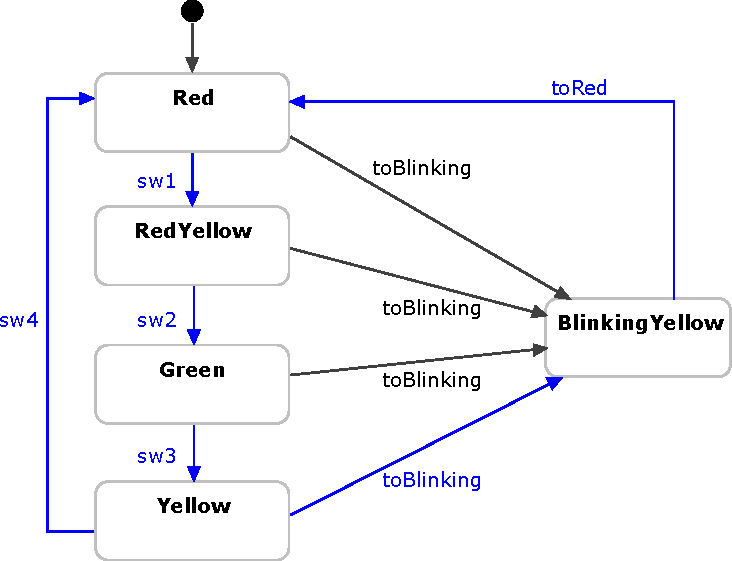
\includegraphics[scale=0.7]{modellek-ellenorzese/figures/pic_fedettseg-jelzolampa-pelda.pdf}
	\end{center}
	
Vegyük az alábbi, két tesztesetből álló tesztkészletet (az elfogadási kritérium nem lényeges a fedettség szempontjából, így azt elhagytuk):

\begin{center}
	\begin{tabular}{rl}\toprule
		Teszteset & Bemenet (\code{n}) \\ \midrule
		1 & \code{sw1}, \code{sw2}, \code{sw3}, \code{sw4} \\ %\hline
		2 & \code{sw1}, \code{sw2}, \code{sw3}, \code{toBlinking}, \code{toRed} \\ \bottomrule
	\end{tabular}
\end{center}

Ez a két teszt az összes állapotot be fogja járni. Így az állapotgépben az \emph{állapotfedettség} $\frac{5}{5} = 1 = 100 \%$.

Ugyanakkor ez a tesztkészlet mégsem érzékeny minden hibára. Nem tudnánk kimutatni például, ha az implementációban kifelejtenénk a \allapot{RedYellow}-ból \allapot{BlinkingYellow}-ba vezető tranzíciót. Ez azért van, mert bár az állapotfedettség teljes, az átmenetfedettség nem. Összesen 9 tranzíció található az állapotgépben, ebből 6-ot fed le a két teszteset együtt (kékkel jelölt átmenetek), így az \emph{átmenetfedettség} $\frac{6}{9} = 0{,}666 = 66{,}6 \%$.

Fontos megjegyezni, hogy ha elérnénk néhány új teszteset definiálásával a teljes átmenetfedettséget, az sem feltétlen lenne képes kimutatni minden lehetséges hibát. Ha például az implementációban -- hibásan -- szerepelne egy \allapot{Green} állapotból \allapot{Red} állapotba vezető átmenet, azt nem feltétlen tudnánk kimutatni egy (a specifikáción) teljes fedettséget elérő tesztkészlettel sem.
\end{pelda}

A fenti áttekintésből az is látszik, hogy egy magas fedettségi arány csak szükséges, de nem elégséges feltétele a jó minőségű rendszer fejlesztésének. Gyakran ez a szám félrevezető is lehet, illetve rossz irányba viheti a teszttervezést.


\section{Tesztelés futásidőben (futásidejű verifikáció)}\label{sec:futasideju-verifikacio}
Ebben a fejezetben a futásidejű ,,öntesztelés'' vagy monitorozás alapötletét mutatjuk be. Bizonyos esetekben kiemelkedően magas minőségi elvárásaink vannak a rendszerünkkel szemben (pl. biztonságkritikus alkalmazási területek). Más esetekben olyan külső komponenseket használunk, amelyek minőségéről nem tudunk alaposan meggyőződni (pl. egy lefordított, más által fejlesztett alkalmazást csak korlátozottan tudunk tesztelni). Ilyenkor az elvárásaink egy részét elhelyezzük magában a megvalósított rendszerben és folyamatosan vizsgáljuk. Azokat a követelményeket, amelyek teljesülését folyamatosan, minden állapotban elvárjuk, \fogalomragozva{invarians}{invariánsoknak} nevezzük.

A monitorozás általános elrendezését szemlélteti \aref{fig:monitorozas-elrendezes}.~ábra.

\begin{figure}[h]
	\centering
	\input{modellek-ellenorzese/figures/monitorozas-elrendezes.pdf_tex}
	
	\caption{A monitorozás általános elrendezése}
	\label{fig:monitorozas-elrendezes}
\end{figure}

A monitorozás két fő lépésből áll:
\begin{itemize}
\item \emph{bemenetek ellenőrzéséből}, amely során a bemeneti adatok megfelelőségét vizsgáljuk a definiált bemeneti invariánsok (előfeltételek) alapján, és/vagy
\item \emph{hihetőségvizsgálatból}, amely során a kimeneti adatok megfelelőségét vizsgáljuk a bemeneti adatok és a definiált kimeneti invariánsok (utófeltételek) alapján.
\end{itemize}

Egyes esetekben az invariánsok igen egyszerűek (például egy valós számok négyzetre emelést megvalósító függvény végén vizsgálhatjuk, hogy a kapott eredmény negatív-e; a negatív eredményt hibásnak minősítjük). Ilyenkor tipikusan az implementáció is három részre tagolódik, követve \aref{fig:monitorozas-elrendezes}.~ábrán látható elrendezést:
\begin{itemize}
\item Először az \emph{előfeltételt} vizsgáljuk. Ha ez nem teljesül, kivételről beszélünk. Ez egy normálistól eltérő, váratlan helyzet, aminek a kezelését máshol valósítjuk meg (ilyen körülmények közt az implementációnk helyességét nem követeljük meg). Ha az előfeltétel nem teljesül, annak oka a rendszer hibás használata (nem megfelelő bemeneti adatokat kapott).
\item Amennyiben az előfeltétel teljesült, megtörténik az érdemi logika \emph{végrehajtása}.
\item A végrehajtás után az utófeltétel vizsgálatára kerül sor. Amennyiben az utófeltétel nem teljesül, olyan hibás állapotba került a rendszer, amely kezelésére nincs felkészítve. Ennek oka lehet a hibás implementáció vagy futásidejű hiba.
\end{itemize}

\begin{pelda}
Az alábbi példakód egy másodfokú egyenlet gyökeit számolja ki:

\begin{lstlisting}[language=C++]
void Roots(float a, b, c, float &x1, &x2) {
    float d = sqrt(b*b-4*a*c);

    x1 = (-b+d)/(2*a);
    x2 = (-b-d)/(2*a);
}
\end{lstlisting}

Tudhatjuk, hogy ez a kód nem működik helyesen minden esetben. Feltételezzük, hogy a diszkrimináns ($D=b^2-4\cdot a\cdot c$) nemnegatív, különben a gyökvonást negatív számon végezzük el. Tudjuk azt is, hogy a kiszámított $x_1$ és $x_2$ értékeknek zérushelyeknek kell lennie, azaz elvárt, hogy $ax_1^2 + bx_1 + c = 0$ és $ax_2^2 + bx_2 + c = 0$. Ezekkel az elő- és utófeltételekkel kiegészíthetjük az implementációt is az alábbiak szerint:


\begin{lstlisting}[language=C++,morekeywords={assert}]
void RootsMonitor(float a, b, c, float &x1, &x2) {
    // el(*@\textcolor{commentcolor}{ő}@*)feltétel
    float D = b*b-4*a*c;
    if (D < 0)
        throw "Invalid input!";

    // végrehajtás
    Roots(a, b, c, x1, x2);

    // utófeltétel
    assert(a*x1*x1+b*x1+c == 0 && a*x2*x2+b*x2+c == 0);
}
\end{lstlisting}
\end{pelda}

Monitorozást nem csak ilyen egyszerű esetekben lehet használni, összetett monitorok is elképzelhetők. Például állapotgépek esetén készíthetünk egy monitor régiót, ami a rendszer megvalósításával párhuzamosan fut és detektálja a hibás vagy tiltott állapotokat, akciókat.

\begin{megjegyzes}
Az elő- és utófeltételek adják az ún. \emph{design by contract} elv alapötletét. Ennek célja a rendszer minőségének javítása (a hibák elkerülése) azáltal, hogy a rendszer minden komponensére elő- és utófeltételeket határozunk meg. Egy adott $x$ komponenst felhasználó $y$ komponensnek garantálnia kell, hogy $x$ előfeltételei teljesülnek a felhasználáskor, cserébe feltételezheti, hogy a válasz teljesíteni fogja $x$ utófeltételeit. A másik oldalról $x$ feltételezi, hogy az előfeltételei teljesülni fognak, és az ő felelőssége az utófeltételek teljesítése. Egy komponensre az elő- és utófeltételek összességét \emph{szerződésnek} hívjuk, amely lényegében az adott komponens egy specifikációja. A legtöbb programozási nyelv beépítve vagy kiegészítéseken keresztül támogatást nyújt a szerződések precíz leírásához és esetleg azok automatikus ellenőrzéséhez is.
\end{megjegyzes}





\section{Formális verifikáció\kieg}\label{sec:formalis-verifikacio}
\Fogalom{formalis-verifikacio} alatt olyan módszereket értünk, amelyek segítségével adott modellek vagy programok helyességét matematikailag precíz eszközökkel vizsgálhatjuk. Három fontosabb formális verifikációs módszert (családot) említünk meg:
\begin{itemize}
\item Modellellenőrzés;
\item Automatikus helyességbizonyítás, amely során axiómarendszerek alapján tételbizonyítás segítségével próbáljuk a helyességet belátni;
\item Konformanciavizsgálat, amely során adott modellek közt bizonyos konformanciarelációk teljesülését vizsgáljuk, így beláthatjuk, hogy különböző modellek viselkedése megegyező vagy eltérő az adott relációk szerint.
\end{itemize}

Jelen jegyzetben kitekintésként a modellellenőrzést mutatjuk be röviden. Bővebben a formális verifikációról a \form (BMEVIMIM100) MSc tárgy\footnote{\url{https://inf.mit.bme.hu/edu/courses/form}} keretei közt szólunk.

\paragraph{Modellellenőrzés.}
A \fogalom{modellellenorzes} egy olyan módszer, amelynek során egy adott modellen vagy implementáción egy követelmény teljesülését vizsgáljuk. A modellellenőrzés egyik előnye, hogy amennyiben a követelmény nem teljesül, lehetséges egy ellenpéldát adni. Az \fogalom{ellenpelda} egy olyan futási szekvencia, amely megmutatja, hogyan lehetséges a vizsgált követelményt megsérteni. Ez nagyban segíthet a hibás működés okának meghatározásában.

A modellellenőrzés -- a teszteléssel szemben -- egy \emph{teljes} módszer, azaz az adott modell vizsgálata kimerítő. Ennek következtében lehetőség van a helyes működés bizonyítására is, míg ez teszteléssel nem lehetséges. Ugyanakkor a modellellenőrzés igen nagy számítási igényű, ezért használhatósága korlátozott.



\section{Kapcsolódó témák}
\textbf{TODO}

\section{Gyakorlati jelentőség}
Mint azt már a fejezet elején említettük, az informatikának, mint mérnöki diszciplínának kulcsfontosságú része az elkészített munka ellenőrzése, legyen az specifikáció vagy implementáció. Minél nagyobb az elkészített rendszer kritikussága, annál nagyobb a fejlesztés folyamán az ellenőrzése szerepe.

Manapság már szinte elképzelhetetlen egy modern fejlesztőkörnyezet beépített statikus ellenőrzés nélkül. Elérhetők további, igen kifinomult eszközök, amelyek statikus ellenőrzés segítségével felhívhatják a figyelmet hibákra vagy veszélyes konstrukciókra. 

Az általunk írt implementáció nem tekinthető befejezettnek, amíg nem terveztünk és implementáltunk hozzá egy megfelelő tesztkészletet. Természetesen nem csak a megfelelően releváns tesztkészlet megvalósítása az elvárás: az implementációnkon a teszteknek sikeresnek kell lenniük ahhoz, hogy a fejlesztés következő fázisára továbbléphessünk, legyen az akár az integráció, akár a megrendelőnek történő átadás.

Különösen kritikus esetekben, például egy repülő vagy egy atomerőmű vezérlőrendszerénél, netán orvosi eszközök beágyazott szoftvereinél a tesztelés ismertetett hibái túlzott kockázatot hordozhatnak, ezért gyakran kiegészül a tervek és a megvalósítás vizsgálata formális módszerek használatával.

\subsection{Kapcsolódó eszközök}
Ebben a szakaszban néhány olyan (többnyire jól ismert és ingyenes) eszközt sorolunk fel, amely a gyakorlatban megvalósítja a bemutatott módszerek némelyikét.

Egyszerűbb statikus analízis eszközöket beépítve találhatunk a fejlettebb fejlesztőeszközökben (pl. Eclipse\footnote{\url{http://eclipse.org}}) és modellező eszközökben (pl. Yakindu). Ezeken kívül számos, mélyebb analízist lehetővé tevő eszköz létezik. C esetén gyakran használatos a Lint stb. nyelv esetén a Cppcheck\footnote{\url{http://cppcheck.sourceforge.net/}} és cpplint\footnote{\url{https://github.com/google/styleguide/tree/gh-pages/cpplint}} eszközök. Java nyelvű programok statikus ellenőrzésére használható például a FindBugs\footnote{\url{http://findbugs.sourceforge.net/}} vagy a PMD\footnote{\url{http://pmd.github.io/}} eszköz. A Coverity cég C, \cpp és Java nyelvű programok statikus ellenőrzésére kínál megoldást, amelyek közül például a Coverity Scan\footnote{\url{http://www.coverity.com/products/coverity-scan/}} nyílt forráskódú programokra ingyenesen használható.

C és \cpp nyelvű programokhoz használható tesztfuttató keretrendszer például a Google Test\footnote{\url{https://github.com/google/googletest}}. Java programok modultesztelését segítheti például a JUnit\footnote{\url{http://junit.org/}} keretrendszer.

C és \cpp nyelvű szoftverek modellellenőrzésre jól használható például a CBMC\footnote{\url{http://www.cprover.org/cbmc/}} eszköz. ,,Állapotgép-jellegű'' modellek esetén jó választás lehet az UPPAAL\footnote{\url{http://www.uppaal.org/}} vagy a nuXmv\footnote{\url{https://nuxmv.fbk.eu/}} eszközök használata.

\section{Tanulást segítő anyagok}

\subsection{Ellenőrző kérdések}
\begin{itemize}
	\item  \textbf{TODO}
	\item
	\item
\end{itemize}

%\subsection{Kulcsfogalmak}
%\textbf{TODO}

%\subsection{Szójegyzék}
%\textbf{TODO}